% questions.tex —— 2004 年·普通高等学校招生考试·福建卷·理科 · 题目内容片段（无答案）
% 由 tools/generate_projects.py 依来源总账自 2004/2004_数学真题_福建理科_试题.md 生成，勿手改（改源 MD 后重跑）

\gkpart{一、选择题：本大题共 12 小题，每小题 5 分，共 60 分．在每小题给出的四个选项中，只有一项是符合题目要求的．}

\begin{question}
\gkti{1}复数 $\left(\dfrac{1-\mathrm{i}}{1+\mathrm{i}}\right)^{10}$ 的值是\mbox{（　　）}

\begin{gkopts}(4)
\task A．$-1$
\task B．$1$
\task C．$-32$
\task D．$32$
\end{gkopts}

\end{question}
\begin{question}
\gkti{2}$\tan 15^\circ + \cot 15^\circ$ 的值是\mbox{（　　）}

\begin{gkopts}(2)
\task A．$2$
\task B．$2 + \sqrt{3}$
\task C．$4$
\task D．$\dfrac{4\sqrt{3}}{3}$
\end{gkopts}

\end{question}
\begin{question}
\gkti{3}命题 $p$：若 $a, b \in \mathbf{R}$，则 $|a| + |b| > 1$ 是 $|a + b| > 1$ 的充要条件．命题 $q$：函数 $y = \sqrt{|x - 1| - 2}$ 的定义域是 $(-\infty, -1] \cup [3, +\infty)$．则\mbox{（　　）}

\begin{gkopts}(2)
\task A．“$p$ 或 $q$”为假
\task B．“$p$ 且 $q$”为真
\task C．$p$ 真 $q$ 假
\task D．$p$ 假 $q$ 真
\end{gkopts}

\end{question}
\begin{question}
\gkti{4}已知 $F_1, F_2$ 是椭圆的两个焦点，过 $F_1$ 且与椭圆长轴垂直的直线交椭圆于 $A, B$ 两点，若 $\triangle ABF_2$ 是正三角形，则这个椭圆的离心率是\mbox{（　　）}

\begin{gkopts}(2)
\task A．$\dfrac{\sqrt{2}}{3}$
\task B．$\dfrac{\sqrt{3}}{3}$
\task C．$\dfrac{\sqrt{2}}{2}$
\task D．$\dfrac{\sqrt{3}}{2}$
\end{gkopts}

\end{question}
\begin{question}
\gkti{5}已知 $m, n$ 是不重合的直线，$\alpha, \beta$ 是不重合的平面，有下列命题：

① 若 $m \subset \alpha$，$n \parallel \alpha$，则 $m \parallel n$；

② 若 $m \parallel \alpha$，$m \parallel \beta$，则 $\alpha \parallel \beta$；

③ 若 $\alpha \cap \beta = n$，$m \parallel n$，则 $m \parallel \alpha$ 且 $m \parallel \beta$；

④ 若 $m \perp \alpha$，$m \perp \beta$，则 $\alpha \parallel \beta$．

其中真命题的个数是\mbox{（　　）}

\begin{gkopts}(4)
\task A．$0$
\task B．$1$
\task C．$2$
\task D．$3$
\end{gkopts}

\end{question}
\begin{question}
\gkti{6}某校高二年级共有六个班级，现从外地转入 $4$ 名学生，要安排到该年级的两个班级且每班安排 $2$ 名，则不同的安排方案种数为\mbox{（　　）}

\begin{gkopts}(2)
\task A．$\mathrm{A}_6^2 \mathrm{C}_4^2$
\task B．$\dfrac{1}{2}\mathrm{A}_6^2 \mathrm{C}_4^2$
\task C．$\mathrm{A}_6^2 \mathrm{A}_4^2$
\task D．$2\mathrm{A}_6^2$
\end{gkopts}

\Needspace{0.4\textheight}
\end{question}
\begin{question}
\gkti{7}已知函数 $y = \log_2 x$ 的反函数是 $y = f^{-1}(x)$，则函数 $y = f^{-1}(1 - x)$ 的图象是\mbox{（　　）}
\nopagebreak[4]
\begin{center}% 来源：固定来源 PDF（2004福建理.pdf）第 1 页（印刷页 164）Q7 四选项图
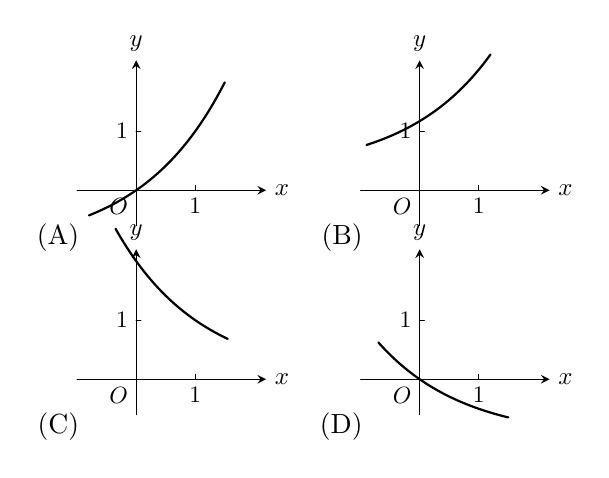
\begin{tikzpicture}[x=0.75cm, y=0.75cm, >=stealth, line cap=round, line join=round]
  \tikzset{
    axis/.style={->, thin},
    curve/.style={thick},
    tick/.style={thin}
  }

  % (A)
  \begin{scope}[shift={(0, 3.2)}]
    \draw[axis] (-1.0, 0) -- (2.2, 0) node[right, scale=0.9] {$x$};
    \draw[axis] (0, -0.6) -- (0, 2.2) node[above, scale=0.9] {$y$};
    \node[below left, scale=0.85] at (0, 0) {$O$};
    \draw[tick] (1, 0) -- (1, 0.08);
    \node[below, scale=0.85] at (1, 0) {$1$};
    \draw[tick] (0, 1) -- (0.08, 1);
    \node[left, scale=0.85] at (0, 1) {$1$};
    \draw[curve, domain=-0.8:1.5, samples=50] plot (\x, {2^(\x) - 1});
    \node[below left] at (-0.8, -0.4) {(A)};
  \end{scope}

  % (B)
  \begin{scope}[shift={(4.8, 3.2)}]
    \draw[axis] (-1.0, 0) -- (2.2, 0) node[right, scale=0.9] {$x$};
    \draw[axis] (0, -0.6) -- (0, 2.2) node[above, scale=0.9] {$y$};
    \node[below left, scale=0.85] at (0, 0) {$O$};
    \draw[tick] (1, 0) -- (1, 0.08);
    \node[below, scale=0.85] at (1, 0) {$1$};
    \draw[tick] (0, 1) -- (0.08, 1);
    \node[left, scale=0.85] at (0, 1) {$1$};
    \draw[curve, domain=-0.9:1.2, samples=50] plot (\x, {2^(\x - 0.2) + 0.3});
    \node[below left] at (-0.8, -0.4) {(B)};
  \end{scope}

  % (C)
  \begin{scope}[shift={(0, 0)}]
    \draw[axis] (-1.0, 0) -- (2.2, 0) node[right, scale=0.9] {$x$};
    \draw[axis] (0, -0.6) -- (0, 2.2) node[above, scale=0.9] {$y$};
    \node[below left, scale=0.85] at (0, 0) {$O$};
    \draw[tick] (1, 0) -- (1, 0.08);
    \node[below, scale=0.85] at (1, 0) {$1$};
    \draw[tick] (0, 1) -- (0.08, 1);
    \node[left, scale=0.85] at (0, 1) {$1$};
    \draw[curve, domain=-0.35:1.55, samples=50] plot (\x, {2^(1 - \x)});
    \node[below left] at (-0.8, -0.4) {(C)};
  \end{scope}

  % (D)
  \begin{scope}[shift={(4.8, 0)}]
    \draw[axis] (-1.0, 0) -- (2.2, 0) node[right, scale=0.9] {$x$};
    \draw[axis] (0, -0.6) -- (0, 2.2) node[above, scale=0.9] {$y$};
    \node[below left, scale=0.85] at (0, 0) {$O$};
    \draw[tick] (1, 0) -- (1, 0.08);
    \node[below, scale=0.85] at (1, 0) {$1$};
    \draw[tick] (0, 1) -- (0.08, 1);
    \node[left, scale=0.85] at (0, 1) {$1$};
    \draw[curve, domain=-0.7:1.5, samples=50] plot (\x, {2^(-\x) - 1});
    \node[below left] at (-0.8, -0.4) {(D)};
  \end{scope}
\end{tikzpicture}
\end{center}
\nopagebreak[4]
\end{question}
\begin{question}
\gkti{8}已知 $\vec{a}, \vec{b}$ 是非零向量且满足 $(\vec{a} - 2\vec{b}) \perp \vec{a}$，$(\vec{b} - 2\vec{a}) \perp \vec{b}$，则 $\vec{a}$ 与 $\vec{b}$ 的夹角是\mbox{（　　）}

\begin{gkopts}(2)
\task A．$\dfrac{\pi}{6}$
\task B．$\dfrac{\pi}{3}$
\task C．$\dfrac{2\pi}{3}$
\task D．$\dfrac{5\pi}{6}$
\end{gkopts}

\end{question}
\begin{question}
\gkti{9}若 $(1 - 2^x)^9$ 展开式的第 $3$ 项为 $288$，则 $\lim\limits_{n \to \infty} \left(\dfrac{1}{x} + \dfrac{1}{x^2} + \dots + \dfrac{1}{x^n}\right)$ 的值是\mbox{（　　）}

\begin{gkopts}(4)
\task A．$2$
\task B．$1$
\task C．$\dfrac{1}{2}$
\task D．$\dfrac{2}{5}$
\end{gkopts}

\Needspace{0.4\textheight}
\end{question}
\begin{question}
\gkti{10}如图，$A, B, C$ 是表面积为 $48\pi$ 的球面上三点，$AB = 2$，$BC = 4$，$\angle ABC = 60^\circ$，$O$ 为球心，则直线 $OA$ 与截面 $ABC$ 所成的角是\mbox{（　　）}

\begin{gkopts}(2)
\task A．$\arcsin\dfrac{\sqrt{3}}{6}$
\task B．$\arccos\dfrac{\sqrt{3}}{6}$
\task C．$\arcsin\dfrac{\sqrt{3}}{3}$
\task D．$\arccos\dfrac{\sqrt{3}}{3}$
\end{gkopts}
\nopagebreak[4]
\begin{center}% 来源：固定来源 PDF（2004福建理.pdf）第 1 页（印刷页 164）Q10 球面截面示意图
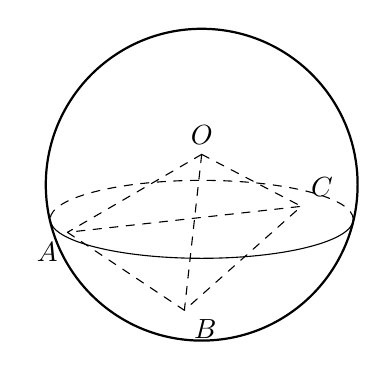
\begin{tikzpicture}[scale=1.1, line cap=round, line join=round]
  % 球体轮廓
  \draw[thick] (0, 0) circle (1.8);

  % 截面圆轮廓（前实后虚）
  \draw[dashed, thin] (1.75, -0.4) arc[start angle=0, end angle=180, x radius=1.75, y radius=0.45];
  \draw[thin] (-1.75, -0.4) arc[start angle=180, end angle=360, x radius=1.75, y radius=0.45];

  % 关键点坐标
  \coordinate (O) at (0, 0.35);
  \coordinate (A) at (-1.55, -0.55);
  \coordinate (B) at (-0.2, -1.45);
  \coordinate (C) at (1.15, -0.25);

  % 三角形 ABC 虚线
  \draw[dashed] (A) -- (B) -- (C) -- cycle;

  % OA, OB, OC 连线虚线
  \draw[dashed] (O) -- (A);
  \draw[dashed] (O) -- (B);
  \draw[dashed] (O) -- (C);

  % 顶点标注
  \node[above] at (O) {$O$};
  \node[below left] at (A) {$A$};
  \node[below right] at (B) {$B$};
  \node[above right] at (C) {$C$};
\end{tikzpicture}
\end{center}
\nopagebreak[4]
\end{question}
\begin{question}
\gkti{11}定义在 $\mathbf{R}$ 上的偶函数 $f(x)$ 满足 $f(x) = f(x + 2)$，当 $x \in [3, 5]$ 时，$f(x) = 2 - |x - 4|$，则\mbox{（　　）}

\begin{gkopts}(1)
\task A．$f\left(\sin\dfrac{\pi}{6}\right) < f\left(\cos\dfrac{\pi}{6}\right)$
\task B．$f(\sin 1) > f(\cos 1)$
\task C．$f\left(\cos\dfrac{2\pi}{3}\right) < f\left(\sin\dfrac{2\pi}{3}\right)$
\task D．$f(\cos 2) > f(\sin 2)$
\end{gkopts}

\Needspace{0.4\textheight}
\end{question}
\begin{question}
\gkti{12}如图，$B$ 地在 $A$ 地的正东方向 $4\text{ km}$ 处，$C$ 地在 $B$ 地的北偏东 $30^\circ$ 方向 $2\text{ km}$ 处，河流的沿岸 $PQ$（曲线）上任意一点到 $A$ 的距离比到 $B$ 的距离远 $2\text{ km}$．现要在曲线 $PQ$ 上选一处 $M$ 建一座码头，向 $B, C$ 两地转运货物．经测算，从 $M$ 到 $B, C$ 两地修建公路的费用分别是 $a$ 万元/$\text{km}$、$2a$ 万元/$\text{km}$，那么修建这两条公路的总费用最低是\mbox{（　　）}

\begin{gkopts}(2)
\task A．$(2\sqrt{7} - 2)a$ 万元
\task B．$5a$ 万元
\task C．$(2\sqrt{7} + 1)a$ 万元
\task D．$(2\sqrt{7} + 3)a$ 万元
\end{gkopts}
\nopagebreak[4]
\begin{center}% 来源：固定来源 PDF（2004福建理.pdf）第 1 页（印刷页 164）Q12 码头选址示意图
\begin{tikzpicture}[scale=1.0, >=stealth, line cap=round, line join=round]
  % 方向标
  \begin{scope}[shift={(-2.2, 1.2)}]
    \draw[->, thin] (0, 0) -- (0, 0.9) node[above] {\small 北};
    \draw[->, thin] (0, 0) -- (0.9, 0) node[right] {\small 东};
  \end{scope}

  % 坐标定义
  \coordinate (A) at (-2.3, -0.5);
  \coordinate (B) at (0.8, -0.5);
  \coordinate (C) at (1.8, 0.9);
  \coordinate (M) at (-0.05, -0.05);
  \coordinate (P) at (0.5, 1.4);
  \coordinate (Q) at (0.3, -1.2);

  % 线段 AB
  \draw[thick] (A) -- (B);

  % 河流沿岸曲线 PQ（双曲线右支一段）
  \draw[thick] (P) to[out=245, in=75] (M) to[out=255, in=105] (Q);

  % 三角形 MBC 公路连线
  \draw (M) -- (B);
  \draw (M) -- (C);
  \draw (B) -- (C);

  % 点标注
  \node[below left] at (A) {$A$};
  \node[below right] at (B) {$B$};
  \node[above right] at (C) {$C$};
  \node[left] at (M) {$M$};
  \node[right] at (P) {$P$};
  \node[right] at (Q) {$Q$};
\end{tikzpicture}
\end{center}
\nopagebreak[4]
\end{question}
\gkpart{二、填空题：本大题共 4 小题，每小题 4 分，共 16 分．把答案填在题中横线上．}

\begin{question}
\gkti{13}直线 $x + 2y = 0$ 被曲线 $x^2 + y^2 - 6x - 2y - 15 = 0$ 所截得的弦长等于 \underline{\hspace{3cm}}．

\end{question}
\begin{question}
\gkti{14}设函数
\nopagebreak[4]
\[
f(x) = \begin{cases} \dfrac{\sqrt{1+x}-1}{x}, & x \neq 0, \\ a, & x = 0, \end{cases}
\]
在 $x = 0$ 处连续，则实数 $a$ 的值为 \underline{\hspace{3cm}}．

\end{question}
\begin{question}
\gkti{15}某射手射击 $1$ 次，击中目标的概率是 $0.9$．他连续射击 $4$ 次，且各次射击是否击中目标相互之间没有影响．有下列结论：

① 他第 $3$ 次击中目标的概率是 $0.9$；

② 他恰好击中目标 $3$ 次的概率是 $0.9^3 \times 0.1$；

③ 他至少击中目标 $1$ 次的概率是 $1 - 0.1^4$．

其中正确结论的序号是 \underline{\hspace{3cm}}．（写出所有正确结论的序号）

\Needspace{0.4\textheight}
\end{question}
\begin{question}
\gkti{16}如图，将边长为 $1$ 的正六边形铁皮的六个角各切去一个全等的四边形，再沿虚线折起，做成一个无盖的正六棱柱容器．当这个正六棱柱容器的底面边长为 \underline{\hspace{3cm}} 时，其容积最大．
\nopagebreak[4]
\begin{center}% 来源：固定来源 PDF（2004福建理.pdf）第 1 页（印刷页 164）Q16 正六棱柱折纸展开图
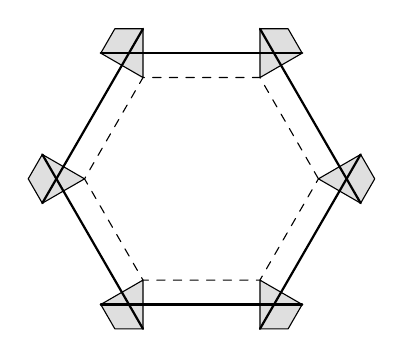
\begin{tikzpicture}[scale=1.1, line cap=round, line join=round]
  \tikzset{
    outer/.style={thick},
    fold/.style={dashed, thin},
    cutout/.style={fill=gray!25, draw=black, thin}
  }

  % 参数：外半径 R=2.0，内半径 r=1.35
  \def\R{2.0}
  \def\r{1.35}

  % 计算切角并填充六个角处的四边形阴影
  \foreach \i in {0, 1, ..., 5} {
    \pgfmathsetmacro{\ang}{\i * 60}
    \pgfmathsetmacro{\prevang}{(\i - 1) * 60}
    \pgfmathsetmacro{\nextang}{(\i + 1) * 60}

    % 外顶点 V
    \coordinate (V\i) at ({\R * cos(\ang)}, {\R * sin(\ang)});
    % 内顶点 W
    \coordinate (W\i) at ({\r * cos(\ang)}, {\r * sin(\ang)});

    % 两侧切口点（从 W 向相邻外边作垂线的垂足）
    \pgfmathsetmacro{\angA}{\ang + 30}
    \pgfmathsetmacro{\dist}{0.5 * (\R - \r)}
    \coordinate (P\i) at ({\R * cos(\ang) - \dist * cos(\ang - 60)}, {\R * sin(\ang) - \dist * sin(\ang - 60)});
    \coordinate (Q\i) at ({\R * cos(\ang) - \dist * cos(\ang + 60)}, {\R * sin(\ang) - \dist * sin(\ang + 60)});

    \filldraw[cutout] (W\i) -- (P\i) -- (V\i) -- (Q\i) -- cycle;
  }

  % 外边界未切除边段
  \foreach \i in {0, 1, ..., 5} {
    \pgfmathsetmacro{\nexti}{int(mod(\i + 1, 6))}
    \draw[outer] (Q\i) -- (P\nexti);
  }

  % 内部虚线折痕（内正六边形）
  \draw[fold] (W0) -- (W1) -- (W2) -- (W3) -- (W4) -- (W5) -- cycle;
\end{tikzpicture}
\end{center}
\nopagebreak[4]
\end{question}
\gkpart{三、解答题：本大题共 6 小题，共 74 分．解答应写出文字说明、证明过程或演算步骤．}

\begin{question}
\gkti{17}（本小题满分 12 分）

设函数 $f(x) = \vec{a} \cdot \vec{b}$，其中向量 $\vec{a} = (2\cos x, 1)$，$\vec{b} = (\cos x, \sqrt{3}\sin 2x)$，$x \in \mathbf{R}$．

（1）若 $f(x) = 1 - \sqrt{3}$ 且 $x \in \left[-\dfrac{\pi}{3}, \dfrac{\pi}{3}\right]$，求 $x$；

（2）若函数 $y = 2\sin 2x$ 的图象按向量 $\vec{c} = (m, n)$（$|m| < \dfrac{\pi}{2}$）平移后得到函数 $y = f(x)$ 的图象，求实数 $m, n$ 的值．

\end{question}
\begin{question}
\gkti{18}（本小题满分 12 分）

甲、乙两人参加一次英语口语考试，已知在备选的 $10$ 道试题中，甲能答对其中的 $6$ 题，乙能答对其中的 $8$ 题．规定每次考试都从备选题中随机抽出 $3$ 题进行测试，至少答对 $2$ 题才算合格．

（1）求甲答对试题数 $\xi$ 的概率分布及数学期望；

（2）求甲、乙两人至少有一人考试合格的概率．

\Needspace{0.4\textheight}
\end{question}
\begin{question}
\gkti{19}（本小题满分 12 分）

在三棱锥 $S - ABC$ 中，$\triangle ABC$ 是边长为 $4$ 的正三角形，平面 $SAC \perp$ 平面 $ABC$，$SA = SC = 2\sqrt{3}$，$M, N$ 分别为 $AB, SB$ 的中点．

（1）证明：$AC \perp SB$；

（2）求二面角 $N - CM - B$ 的大小；

（3）求点 $B$ 到平面 $CMN$ 的距离．
\nopagebreak[4]
\begin{center}% 来源：固定来源 PDF（2004福建理.pdf）第 2 页（印刷页 165）Q19 三棱锥几何示意图
\begin{tikzpicture}[scale=1.1, line cap=round, line join=round]
  % 顶点坐标
  \coordinate (S) at (0.2, 2.5);
  \coordinate (A) at (-1.5, -0.6);
  \coordinate (B) at (2.4, -0.2);
  \coordinate (C) at (-0.3, 0.4);

  % 中点坐标
  \coordinate (M) at ($(A)!0.5!(B)$);
  \coordinate (N) at ($(S)!0.5!(B)$);

  % 虚线边（被遮挡的内侧棱与截面线）
  \draw[dashed] (S) -- (C);
  \draw[dashed] (A) -- (C);
  \draw[dashed] (B) -- (C);
  \draw[dashed] (C) -- (M);
  \draw[dashed] (C) -- (N);

  % 实线边（前侧可见棱）
  \draw[thick] (S) -- (A) -- (B) -- cycle;
  \draw[thick] (M) -- (N);

  % 顶点标签
  \node[above] at (S) {$S$};
  \node[below left] at (A) {$A$};
  \node[right] at (B) {$B$};
  \node[left] at (C) {$C$};
  \node[below] at (M) {$M$};
  \node[above right] at (N) {$N$};
\end{tikzpicture}
\end{center}
\nopagebreak[4]
\end{question}
\begin{question}
\gkti{20}（本小题满分 12 分）

某企业 2003 年的纯利润为 $500$ 万元，因设备老化等原因，企业的生产能力将逐年下降．若不能进行技术改造，预测从今年起每年比上一年纯利润减少 $20$ 万元，今年初该企业一次性投入资金 $600$ 万元进行技术改造，预测在未扣除技术改造资金的情况下，第 $n$ 年（今年为第一年）的利润为 $500\left(1 + \dfrac{1}{2^n}\right)$ 万元（$n$ 为正整数）．

（1）设从今年起的前 $n$ 年，若该企业不进行技术改造的累计纯利润为 $A_n$ 万元，进行技术改造后的累计纯利润为 $B_n$ 万元（须扣除技术改造资金），求 $A_n, B_n$ 的表达式；

（2）依上述预测，从今年起该企业至少经过多少年，进行技术改造后的累计纯利润超过不进行技术改造的累计纯利润？

\end{question}
\begin{question}
\gkti{21}（本小题满分 12 分）

已知 $f(x) = \dfrac{2x - a}{x^2 + 2}$（$x \in \mathbf{R}$）在区间 $[-1, 1]$ 上是增函数．

（1）求实数 $a$ 的值组成的集合 $A$；

（2）设关于 $x$ 的方程 $f(x) = \dfrac{1}{x}$ 的两个非零实根为 $x_1, x_2$．试问：是否存在实数 $m$，使得不等式 $m^2 + tm + 1 \geqslant |x_1 - x_2|$ 对任意 $a \in A$ 及 $t \in [-1, 1]$ 恒成立？若存在，求 $m$ 的取值范围；若不存在，请说明理由．

\end{question}
\begin{question}
\gkti{22}（本小题满分 14 分）

如图，$P$ 是抛物线 $C: y = \dfrac{1}{2}x^2$ 上一点，直线 $l$ 过点 $P$ 且与抛物线 $C$ 交于另一点 $Q$．

（1）若直线 $l$ 与过点 $P$ 的切线垂直，求线段 $PQ$ 中点 $M$ 的轨迹方程；

（2）若直线 $l$ 不过原点且与 $x$ 轴交于点 $S$，与 $y$ 轴交于点 $T$，试求 $\dfrac{|ST|}{|SP|} + \dfrac{|ST|}{|SQ|}$ 的取值范围．

\end{question}